\documentclass[../main.tex]{subfiles}
\graphicspath{{\subfix{../images/}}}


\begin{document}
% RECURRENT NEURAL NETWORKS
%%%%%%%%%%%%%%%%%%%%%%%%%%%%%%%%%%%%%%%%%%%%%%%%%%%%%%%%%%%%%%%%%%%%%%%%%%%%%%%
This section will the fundamental theory to understand the basics of neural networks and a deeper understanding of recurrent neural networks. 

Artificial neural networks was first conceptualized in the 1940s by American psychologist Warren McCulloch and mathematician Walter Pitts, which proposed a model known as the M-P model. The M-P model was a simple functional logic device with limited functionality, but still considered an important start of the theoretical research of neural networks. Frank Rosenblatt, another American psychologist, proposed in 1957 a perceptron model based on the M-P model which created the first true neural network that can learn by adjusting the properties of the network. After a book called \textit{Perceptrons}, published in 1969 by Marvin Minsky and Seymour Papert, the field of artificial neural networks was coerced into a hiatus due to the authors implicating that the perceptron model is limited to simple linearly separable tasks and, therefore, the whole network could not understand the logical relationship of XOR and other linearly inseparable tasks. In the 1980s, American physicist John Hopfield proposed a new type of neural network that sparked new interest in studying neural networks, called a discrete Hopfield network. The potential of the Hopfield neural network encouraged scientist to further develop neural network, which led to the neural networks that exists today \cite{Wu_2017}.
\begin{figure}[H]
\centering
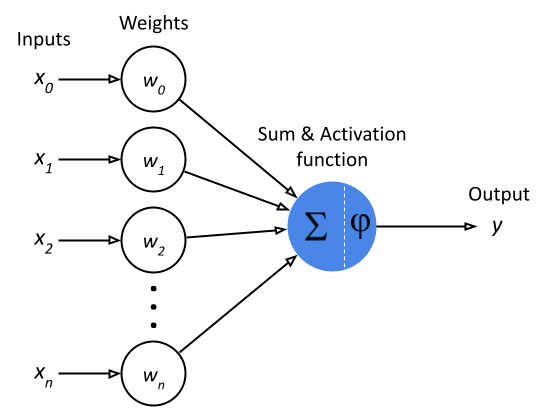
\includegraphics[scale=.5]{artificial-neuron.png}
\caption{An artificial neuron.}
\label{fig:neuron}
\end{figure}
Artificial neural networks (\textit{ANN}) is an artificial representation of the biological brain. The biological brain consists of neurons which communicate with electrical impulses that activates the neuron, creating a response that is the collected sum of all incoming signals. A neuron in the biological brain has many inputs and one output, and the output depends on what the neuron has learned to interpret all the incoming signals as. Combining many neurons creates a network that have the ability to learn by adapting the responses of all neurons in the network. It is the process of learning what to interpret a collection of incoming signals as and output a correct response that makes the network perform well when given a task which the network has learned to perform. A untrained network will have no knowledge of how the neurons should interpret the incomings signals and will therefore be as good as a random guess at the result. The goal of the training is for the network to learn the underlying structure of the data and by learning that, be able to make predictions that are accurate given data the network is not familiar with \cite{Gurney_1997}. It achieves this by adjusting the weights of each input for each neuron and adapting the threshold function, typically done with a technique called gradient descent.

A simple artificial neuron, as seen in Figure \ref{fig:neuron}, consists of $n$ number of inputs $x$. These inputs are multiplied with each associated weight $w$ after which they are summed together and further processed by the activation function. The operation can be expressed as

$$u = \sum_{n=1}^{n}w_n x_n$$

with $u$ being the value that is fed to the activation function. The activation function is what determines at what output $u$ the neuron activates. For example, if the activation function is a step function, anything above a certain threshold $\varphi$ creates a response otherwise the neuron is inactive, and the total input is 0.6 with a threshold of 0.5 the output $y$ of that neuron would be 1. This type of unit is called a threshold logic unit (\textit{TLU}). There are many threshold functions, each with its strengths and weaknesses, and choosing the correct one is dependant on the task the neural network should learn to solve. Step functions can work for classification tasks but does not work for regression tasks where a continuous range of values is the desired output.

\begin{figure}[H]
\centering
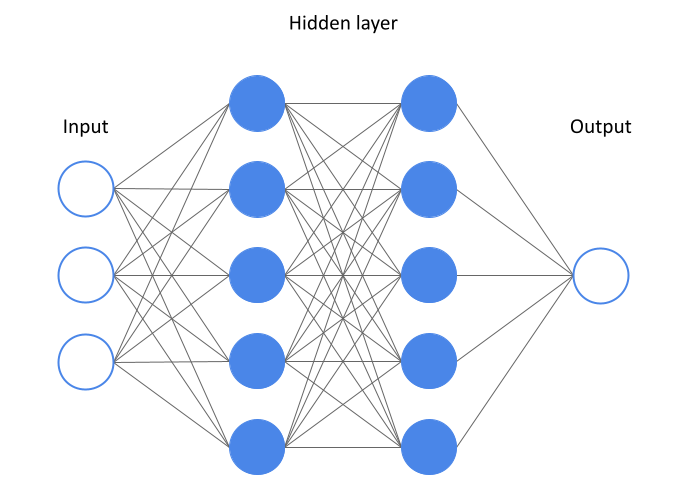
\includegraphics[scale=.4]{nn.png}
\caption{Simple artificial network of three input neurons, two hidden layers with five neurons each and one output neuron.}
\label{fig:network}
\end{figure}

The TLU introduced in this section is one of the simplest form of a artificial neuron and is only suitable for a small set of tasks. A more advanced type of unit is required for the work of this thesis and this type of unit is introduced in section \ref{sec:lstm}.

\subsection{Recurrent neural networks}

Recurrent neural networks (\textit{RNN}) are a class of neural networks that are well suited for time or sequence dependant data. RNNs achieves this by implementing a internal state, \textit{memory}, that can remember temporal dependencies in the data.

Regular feedforward neural networks can predict independent data points that have no relation with the order of the data, for example, classifying images or recognizing patterns. When the order of the data has an impact on the final result, for example, weather forecasts are dependant on what the weather has been the past days or knowing the past trends when predicting stock prices for a specific stock, feedforward neural networks have no way of storing information about past events and can only make a prediction on the current data with no \textit{priori} knowledge \cite{Dipietro_2020, Gupta_2019, Kumara_2021}. Feedforward neural networks process the input to produce an output by a finite series of neurons with no feedback coming from the output to the input \cite{Gurney_1997}. If the network could store information that the weather has been warm the past days, it is more likely to predict the next day is also going to be warm. Regular feedforward neural networks also have the limitation of not being able to process variable length input data.

RNNs are an extension of regular feedforward neural networks that implements hidden  feedback loops within the hidden layers. The feedback loop can be unrolled, which gives a representation similar to a regular feedforward neural network, but each layer is instead a cell that represents one timestep. The depth of a single RNN neuron is equal to the number of timesteps used \cite{di_2018}. Figure \ref{fig:unrolled}, visualizes one recurrent neuron with three timesteps unrolled. RNNs can, contrary to feedforward neural networks, map multiple inputs to multiple outputs, one input to multiple inputs and multiple inputs to one output. For example, $x_1$, $x_2$ and $x_3$ can output only $y_3$, which can be utilized when the result is dependant on a sequence of inputs.

The feedforward operation through the network is used to get the output of the network, the result passing data throught the network. While training, the output of the network is compared with the actual correct value, giving the error of the network. In regular feedforward neural networks, backpropagation is the process of moving backwards through all the layers of the network. For every layer, the partial derivative is calculated of the error for each respective weight, thus, giving the values required for optimizing the weights using a process called gradient descent. Gradient descent is a function that minimizes a given function and the network wants to minimize the error by increasing or decreasing each respective weight, which is achieved by using gradient descent. Because each RNN neuron implements a feedback loop, regular backpropagation is not viable for updating the weights in a RNN, instead a similar method called backpropagation through time (\textit{BPTT}) is utilized. BPTT is an extension of backpropagation, that is able to calculate the derivatives for the RNN neuron. The process can be thought of as unrolling the RNN neuron, which yields a representation similar to that of a layered feedforward network, but instead of layers there are cells. This unrolled representation can then be used to calculate the derivatives which are used to optimize the network by gradient descent.

\begin{figure}[H]
\centering
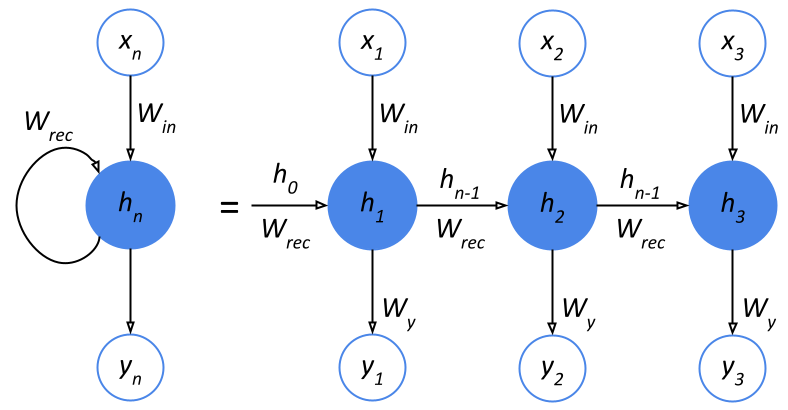
\includegraphics[scale=.4]{rnn-unrolled.png}
\caption{Single RNN neuron with feedback loop on the left and an unrolled RNN neuron with three timesteps on the right.}
\label{fig:unrolled}
\end{figure}

All deep neural networks suffer from gradients that can either explode or vanish \cite{di_2018}. A deep network is any network with multiple layers between the input and the output. The problem is called vanishing or exploding gradients, and is noticeable in regular RNNs, each neuron is a stack of cells similar to a feedforward neural network with multiple layers, making each neuron similar to a deep neural network. Using gradient descent and BPTT to update the weights for each layer and every temporal chain of cells throughout the network, can cause the gradients to either converge to zero or infinite, which consequently, halts the learning process.

The following notation is used in Figure \ref{fig:unrolled} and for the following equations, $x_n$ denotes the input at timestep $n$, $y_n$ denotes the output at timestep $n$, $h_n$ stores the state of the cell, which, gets passed to the next cell, and $h_0$ is set to zero, $W_{in}$ denotes the weight for the input and $W_{rec}$ denotes the weight for the hidden units, $W_y$ denotes the weight for the output. The bias is left out of the equations to simplify them, but would be added to the inner expression in equation \ref{eq:1} as $b_n$.

The output of the cell $h$ at timestep $n$ is calculated as below, $\varphi$ denotes any activation function:
\begin{equation}\label{eq:1}
h_n = \varphi \left( W_{rec} h_{n-1} + W_x x_n \right)
\end{equation}

The output $y$ at timestep $n$ is calculated as:

$$y_n = \varphi \left( W_y h_n \right)$$

Calculating the output of the third cell can, therefore, be expressed as:

$$y_3 = \varphi \left( 
W_y \varphi \left( 
	W_{rec} \varphi \left( 
		W_{rec} \varphi \left( 
			W_{rec} h_{n-3} + W_x x_{n-2} \right)
				+ W_x x_{n-1} \right) 
					+ W_x x_n \right) \right)$$

Product rule to find the gradient for weight $W_{rec}$:

$$\frac{\partial \left( W_{rec} h_{n-1}\right)} {\partial W_{rec}}$$

The output of $y_n$ can be generalized as a series of functions, one for each layer in the network:

$$y_n = f \left( g \left( h \left( \left(x\right) \right) \right) \right)$$

Using the chain rule to calculate the gradient at the first layer $W_1$ can then be expressed as:

$$\frac{\partial y}{\partial W_1} = 
\frac{\partial f}{\partial g}\frac{\partial g}{\partial h} \cdots$$

The gradient of the error for timestep $k$, over T timesteps, can then be expressed as.

\begin{equation}\label{eq:gradienterr}
\frac{\partial E_k}{\partial W} = \frac{\partial E_k}{\partial h_k}\frac{\partial h_k}{\partial C_k}\left( \prod_{n=2}^k  \frac{\partial h_n}{\partial h_{n-1}} \right) \frac{\partial C_1}{\partial W}
\end{equation}

An alternative way of expressing the gradient error on the $k$-th timestep, for $n$ timesteps, using the derivative of $h_n$.

$$\frac{\partial E_k}{\partial W} = \frac{\partial E_k}{\partial h_k}\frac{\partial h_k}{\partial c_k}\left( \prod_{n=2}^k \varphi'\left(W_{rec} h_{n-1} + W_x x_n \right) W_{rec}\right) \frac{\partial h_1}{\partial W}$$

To understand the problem of vanishing and exploding gradients, the equation above can be thought of as a series of repeating functions where the same values are repeatedly multiplied. For the vanishing gradient problem, the weight $W_{rec}$ is multiplied multiple times and if the weight is very small, the value will only decrease more every time it is multiplied. The same is true for the exploding gradient problem, only the value getting multiplied will quickly approach infinity.

\subsubsection{Long Short Term Memory}
\label{sec:lstm}
To solve the problem with long term dependencies and mitigating the vanishing or exploding gradients, \citeauthor{hochreiter_schmidhuber_1997} introduced in 1997, an alternative to regular RNN units called Long Short Term Memory unit or simply LSTM \cite{hochreiter_schmidhuber_1997}.

LSTMs are a unit that replaces the regular cells in an RNN. Compared to a regular cell, LSTM are quite complicated, with multiple pointwise operations, dark blue circles, and learned network layers, light blue rectangles, see Figure \ref{fig:lstm-cell}. The main component of the cell, which enables the cell to perform better than regular RNN cells, is the horizontal line running through the cell at the top, the \textit{cell state}. It allows for information to flow through the cell mostly unchanged, only minor linear operations interacting with the cell state as it moves through the cell. The cell can alter the state of the cell state by a set of carefully regulated gates. The gates are made up of one sigmoid neural net layer and one pointwise multiplication operation. In total, there are three of these gates in the cell and these gates are called the \textit{forget gate}, \textit{input gate} and \textit{output gate}.

\begin{figure}[H]
\centering
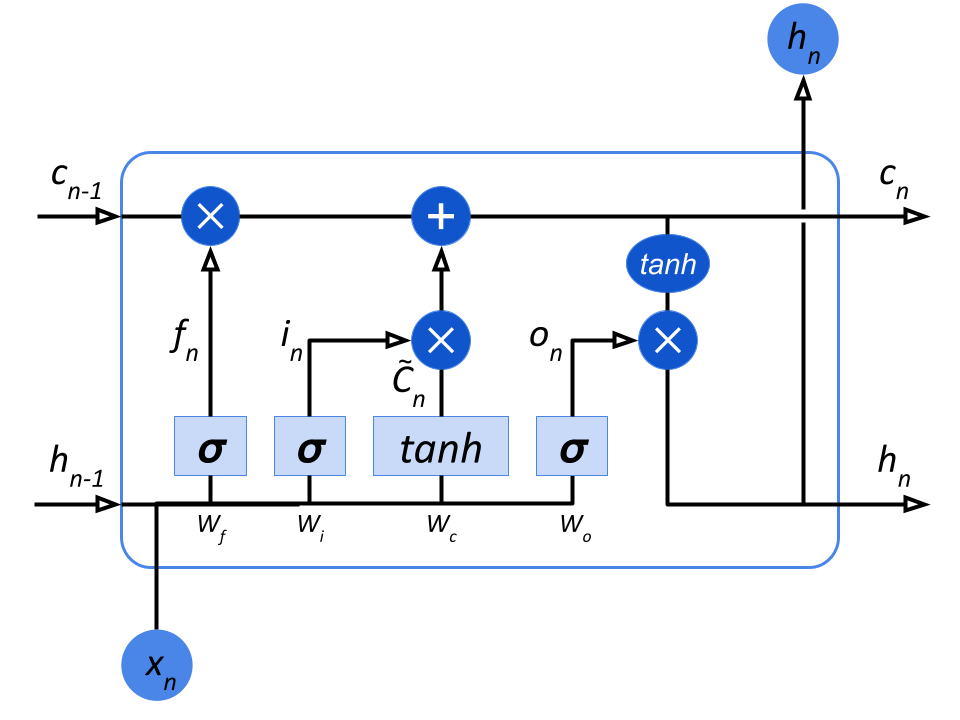
\includegraphics[scale=.4]{lstm-cell.png}
\caption{One LSTM cell with the recurrent cells omitted, source \cite{colah_2015}.}
\label{fig:lstm-cell}
\end{figure}



The forget gate is the first operation in the cell and decides what information to discard given new information. The notation $\left[h_{n-1},x_n \right]$ is used for the input vector.

$$f_n = \sigma \left( W_f \left[h_{n-1},x_n\right] + b_f\right)$$

After the forget gate has decided on what information to discard, the cell decides what new information to store in the cell state. This step is divided into two steps, first, a sigmoid layer decides which values will get updated, handled by the input gate, in Figure \ref{fig:lstm-cell} this is denoted by $i_n$. Then, a new vector of possible values is created by the $\tanh$ layer, denoted by $\tilde{C}_n$.

$$i_n = \sigma \left( W_i\left[ h_{n-1}, x_n \right] + b_i \right)$$

$$\tilde{C}_n = \tanh \left( W_c \left[ h_{n-1}, x_n \right] + b_C\right)$$

The values $i_n$ and $\tilde{C}_n$ are then combined to update the state $C_{n-1}$ to $C_n$. This step is where the cell discards the old information to replace it with the new, according to what was deemed best by the previous steps.

$$C_n = f_n C_{n-1} + i_n \tilde{C}_n$$

Finally, the last step is to output the new information.

$$o_n = \sigma \left( W_o \left[ h_{n-1}, x_n \right] + b_o \right)$$
$$h_n = o_n \tanh\left(C_n\right)$$

The LSTM cell solves the vanishing and exploding gradient problem by making use of the gated internal structure of the cell. The symbol $\cdot$, in equation \ref{eq:lstm}, denotes pointwise multiplication and the symbol $+$ denotes pointwise addition.
\begin{equation} \label{eq:lstm}
C_t = C_{n-1} \cdot f_n + \tilde{C}_n \cdot i_n
\end{equation}

The derivative of equation \ref{eq:lstm}, is equal to the following expression. Note, the $+$ symbol is not the pointwise operation for the following equations.

\begin{equation} \label{eq:lstmder}
\frac{\partial C_n}{\partial C_{n-1}} = \frac{\partial f_n}{\partial C_{n-1}} C_{n-1} + \frac{\partial C_{n-1}}{\partial C_{n-1}} f_n + \frac{\partial i_n}{\partial C_{n-1}} \tilde{C}_n + \frac{\partial \tilde{C}_n}{\partial C_{n-1}} i_n
\end{equation}

The gradient for the LSTM cell can be expressed as an additive gradient as below.

\begin{equation} \label{eq:gradient}
\frac{\partial C_n}{\partial C_{n-1}} = I_n + J_n + K_n + L_n
\end{equation}

Where the equations \ref{eq:A}, \ref{eq:B}, \ref{eq:C} and \ref{eq:D} corresponds to each element in equation \ref{eq:gradient}, which are the derivatives for the four terms in equation \ref{eq:lstmder}.

\begin{equation} \label{eq:A}
I_n = \sigma'\left( W_f \left[ h_{n-1}, x_n \right]\right) W_f o_{n-1} \cdot \tanh'\left( c_{n-1}\right) c_{n-1}
\end{equation}

\begin{equation}\label{eq:B}
J_n = f_n
\end{equation}

\begin{equation} \label{eq:C}
K_n = \sigma'\left( W_i \left[ h_{n-1}, x_n \right]\right) W_i o_{n-1} \cdot \tanh'\left( C_{n-1}\right)\tilde{C}_n
\end{equation}

\begin{equation} \label{eq:D}
L_n = \sigma'\left( W_c \left[ h_{n-1}, x_n \right]\right) W_c o_{n-1} \cdot \tanh'\left( C_{n-1}\right) i_n 
\end{equation}

The LSTM states gradient at timestep $k$ can then be expressed as below, using the equation for calculating the gradient of the error, see equation \ref{eq:gradienterr}.

$$\frac{\partial E_k}{\partial W} = \frac{\partial E_k}{\partial h_k}\frac{\partial h_k}{\partial c_k}\left( \prod_{n=2}^{k}\left[I_n + J_n + K_n + L_n \right] \right) \frac{\partial c_1}{\partial W}$$

Now the gradient is comprised of the forget gate's values, which allows the network to control the gradients values by adjusting the forget gate's parameters at each timestep. By adjusting the parameters of the forget gate, at timestep $n+1$, so that the error gradient does not vanish, the LSTM unit is able to solve the vanishing gradient problem.

One problem that is not solved by regular RNNs or networks using the LSTM unit, is the distribution of the sampling rate of the data points. When the time between each sample is even, the networks thinks that the difference in time is equal, which is true for equally sampled data points. If the samples are not equally sampled, the time difference is thus not equal and, as time is linear, the impact of time on the sample is not linear and the model will have a hard time to understand the impact of each sample.

\subsubsection{Phased LSTM}
The Phased LSTM (\textit{PLSTM}) implementation tested was developed by Francesco Ferroni and is available at \url{https://github.com/fferroni/PhasedLSTM-Keras} (11/03/2022)




\end{document}  